\section*{1. Расчет, используя S-параметры (создание СТЦ1 и СТЦ2 на рабочей частоте)}

В соответствии с заданием, расчет однокаскадного малошумящего усилителя выполняется для рабочей частоты $f = 2.5$ ГГц с использованием линейных S-параметров биполярного транзистора NE68133 (файл Touchstone). 

На первом этапе производится оценка устойчивости транзистора на заданной частоте. В программе HFSS с помощью инструмента Smith Tool на диаграмме Смита строятся окружности устойчивости для входной (S-plane) и выходной (L-plane) плоскостей.

\begin{figure}[H]
	\centering
	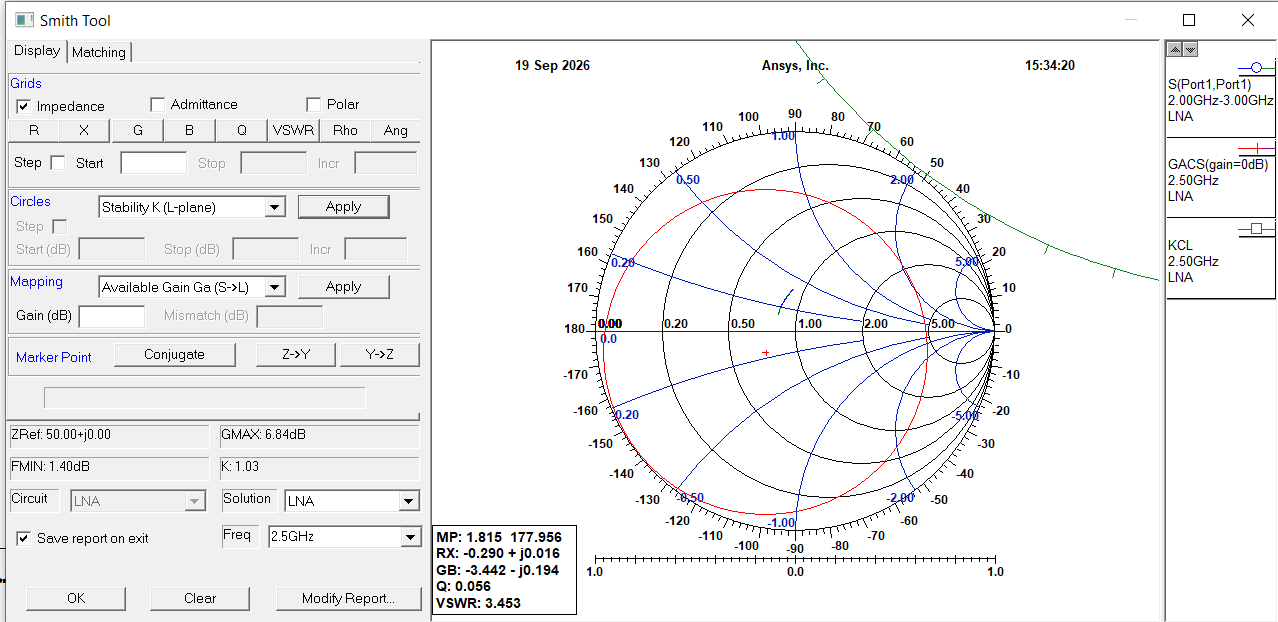
\includegraphics[width=0.8\textwidth]{1.PNG}
	\caption{Окружности устойчивости транзистора на частоте 2.5 ГГц (до стабилизации).}
	\label{fig:stability_before}
\end{figure}

Для обеспечения абсолютной устойчивости каскада (исключения области возможного возбуждения) в цепь эмиттера вводится стабилизирующая индуктивность $L$.

\begin{figure}[H]
	\centering
	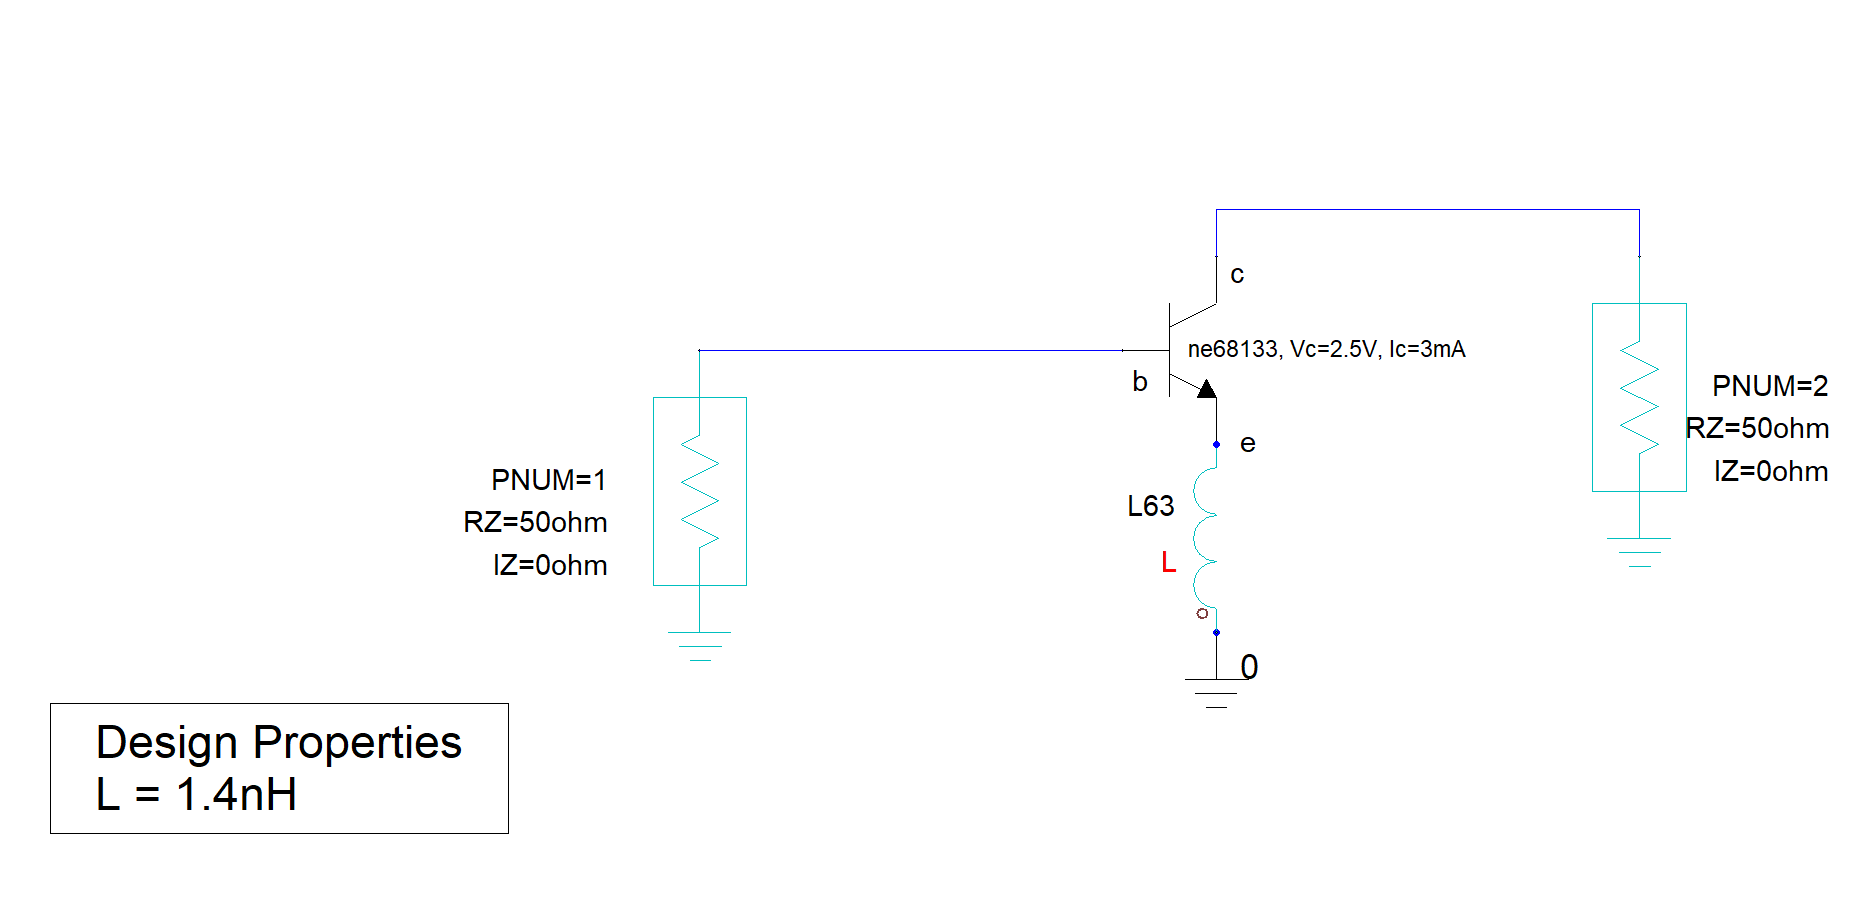
\includegraphics[width=0.7\textwidth]{2.PNG}
	\caption{Схема усилителя с введенной стабилизирующей индуктивностью в цепи эмиттера.}
	\label{fig:sch_with_L}
\end{figure}

Путем параметрической подстройки (тюнинга) номинала данной индуктивности (например, до значения $L = 0.3$ нГн) добиваемся того, чтобы окружности устойчивости полностью вышли за пределы диаграммы Смита, а инвариантный коэффициент устойчивости принял значение $K \ge 1$.

\begin{figure}[H]
	\centering
	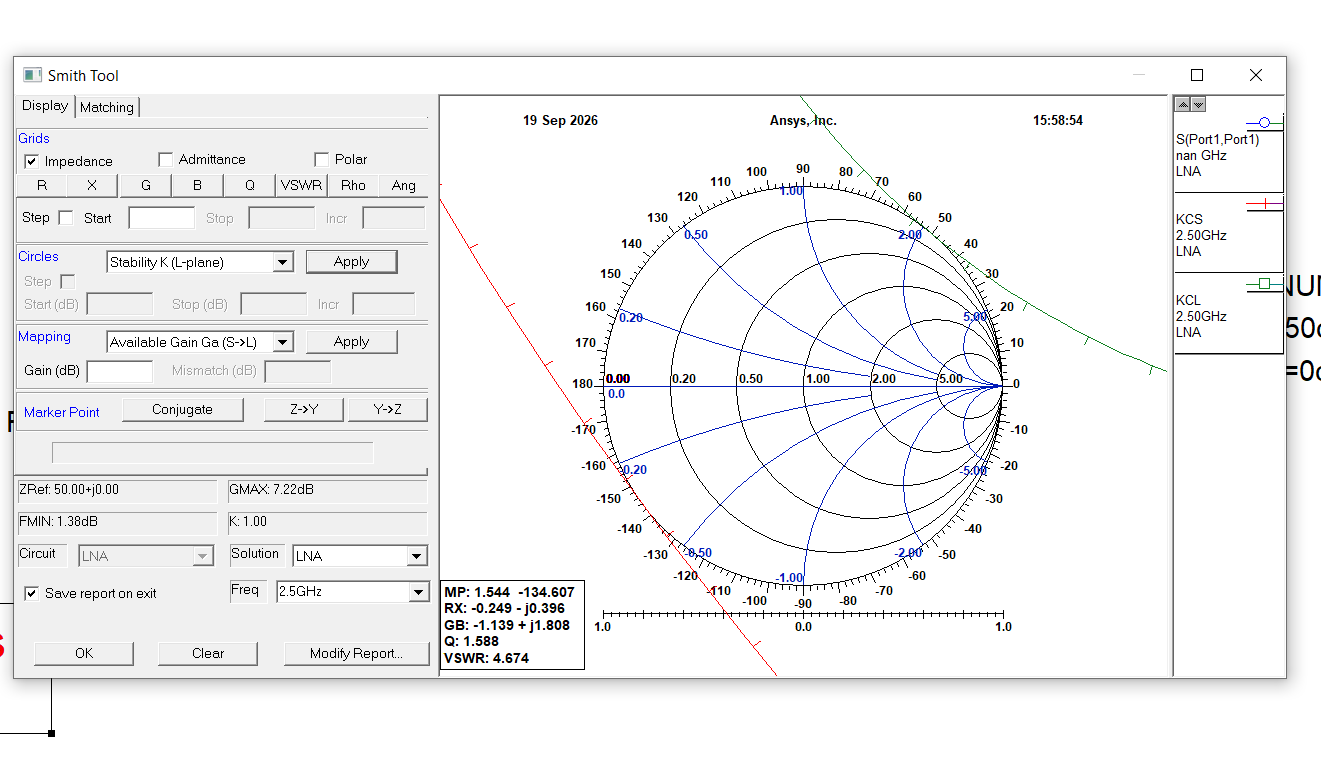
\includegraphics[width=0.8\textwidth]{3.PNG}
	\caption{Изменение положения окружностей устойчивости.}
	\label{fig:stability_tuning_1}
\end{figure}

\begin{figure}[H]
	\centering
	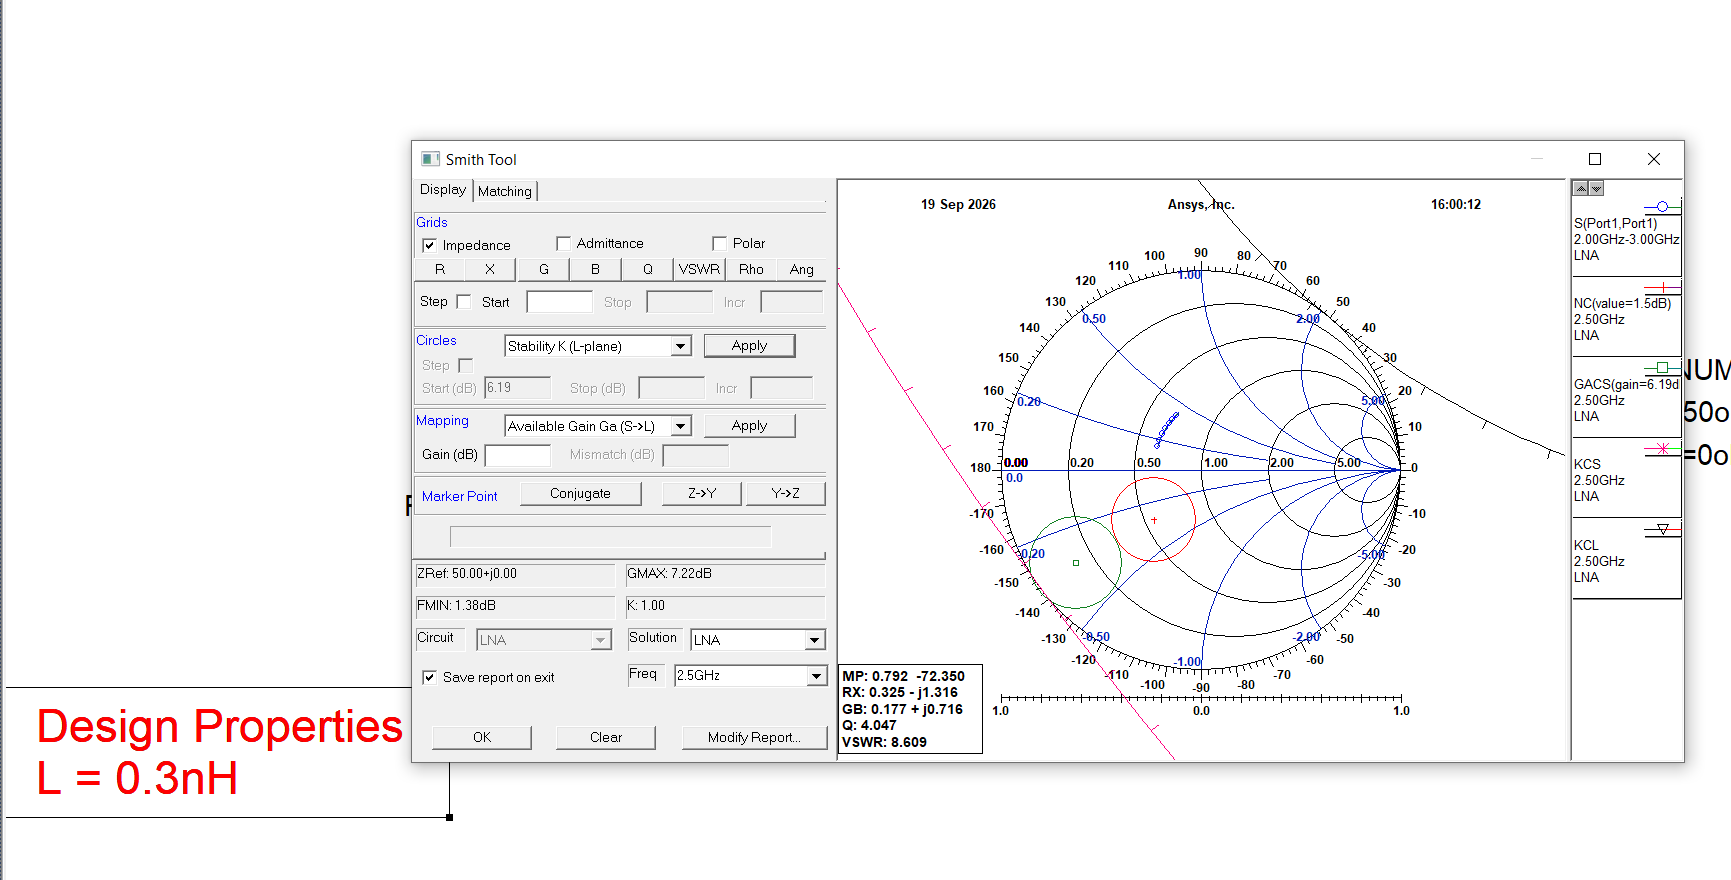
\includegraphics[width=0.8\textwidth]{3_1.PNG}
	\caption{Окружности устойчивости выведены за пределы диаграммы Смита при L = 0.3 нГн.}
	\label{fig:stability_tuning_2}
\end{figure}

После обеспечения абсолютной устойчивости осуществляется синтез входной и выходной согласующих цепей (СТЦ1 и СТЦ2). На диаграмме Смита наносятся окружности равного коэффициента усиления (Available Gain Ga) и равного коэффициента шума (Noise). На пересечении или касании этих окружностей выбирается оптимальная точка $P$, обеспечивающая требуемый компромисс между максимальным усилением и минимальным коэффициентом шума каскада.

\begin{figure}[H]
	\centering
	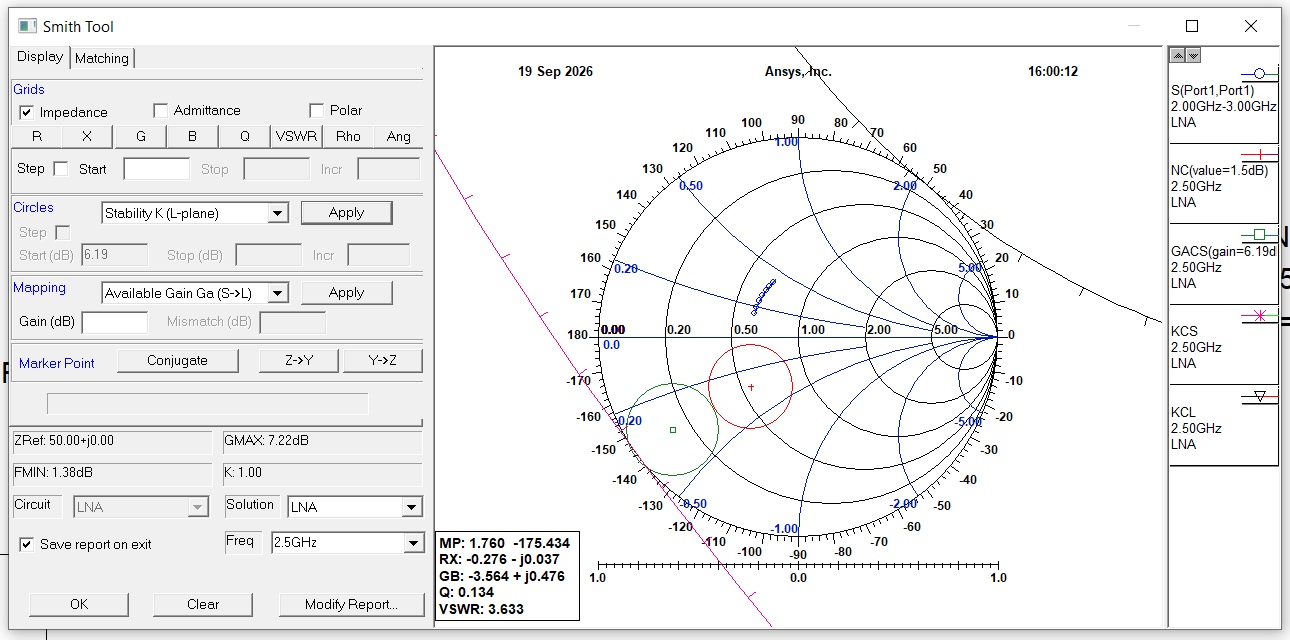
\includegraphics[width=0.8\textwidth]{4.PNG}
	\caption{Окружности равного усиления и шума для выбора оптимальной точки согласования.}
	\label{fig:circles_gain_noise}
\end{figure}

Синтез входной согласующей цепи (СТЦ1) выполняется в плоскости генератора. Путь согласования строится перемещением из центра диаграммы Смита (точка $50$ Ом) в выбранную точку $P$ с помощью добавления идеальных реактивных элементов (например, последовательных и параллельных индуктивностей и емкостей). 

\begin{figure}[H]
	\centering
	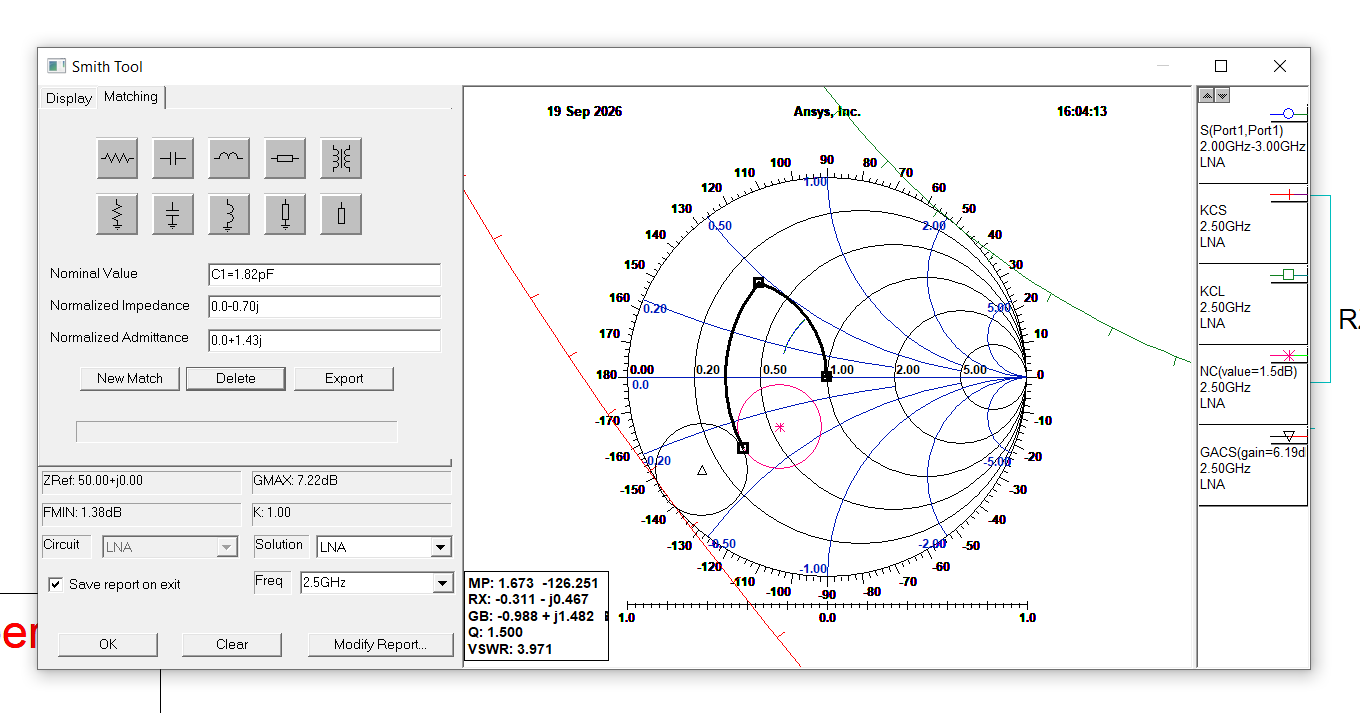
\includegraphics[width=0.8\textwidth]{5.PNG}
	\caption{Синтез входной согласующей цепи (СТЦ1) на диаграмме Смита.}
	\label{fig:match_in}
\end{figure}

Для построения выходной согласующей цепи (СТЦ2) осуществляется пересчет (отображение) выбранной точки $P$ в плоскость нагрузки, в результате чего образуется точка $Q$. Затем на диаграмме находится комплексно-сопряженная точка $Q^*$. Аналогичным образом, с помощью добавления реактивных элементов, производится согласование 50-омной нагрузки с точкой $Q^*$ для обеспечения максимальной передачи мощности на выходе транзистора.

\begin{figure}[H]
	\centering
	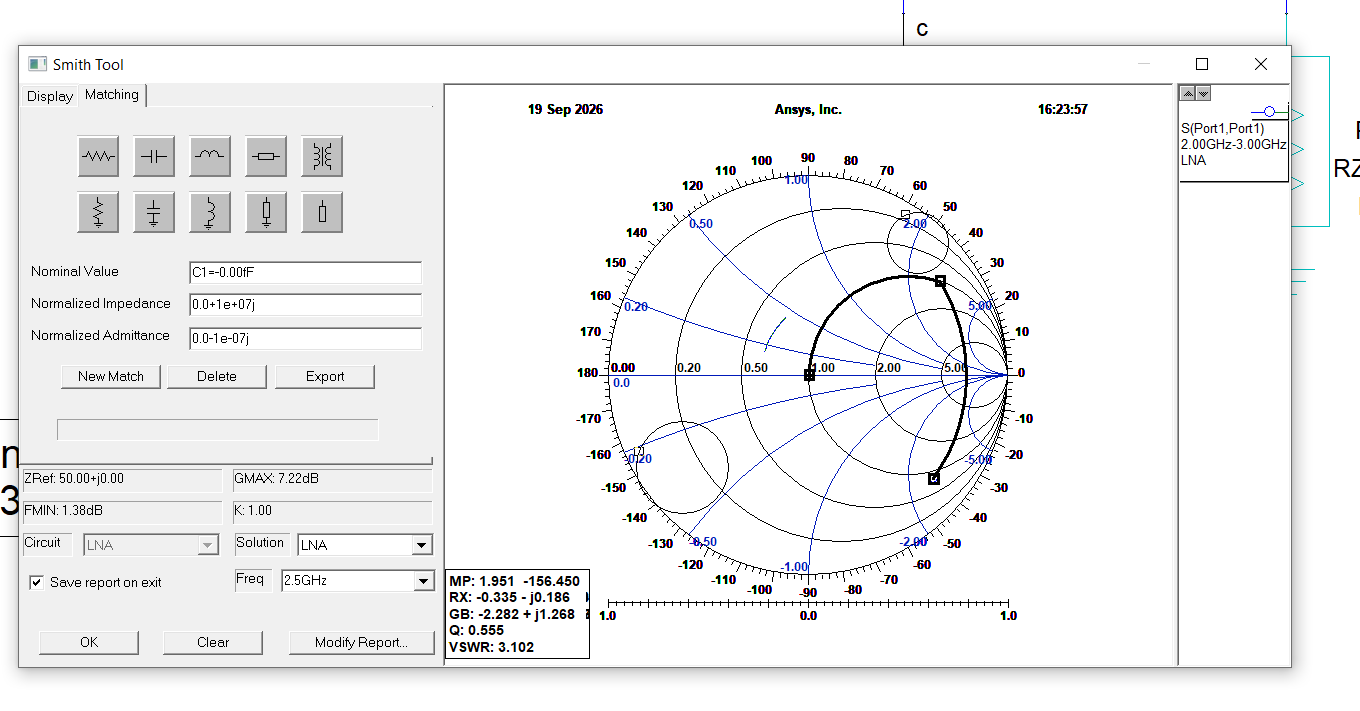
\includegraphics[width=0.8\textwidth]{6.PNG}
	\caption{Синтез выходной согласующей цепи (СТЦ2) на диаграмме Смита.}
	\label{fig:match_out}
\end{figure}

На заключительном этапе созданные подсхемы СТЦ1 и СТЦ2 добавляются в общую схему усилителя в виде блоков, после чего проводится линейный анализ каскада в частотной области. Результаты расчета подтверждают, что на рабочей частоте $f = 2.5$ ГГц достигаются целевые показатели коэффициента передачи $S_{21}$ и обеспечивается приемлемое согласование по портам входа $S_{11}$ и выхода $S_{22}$.

\begin{figure}[H]
	\centering
	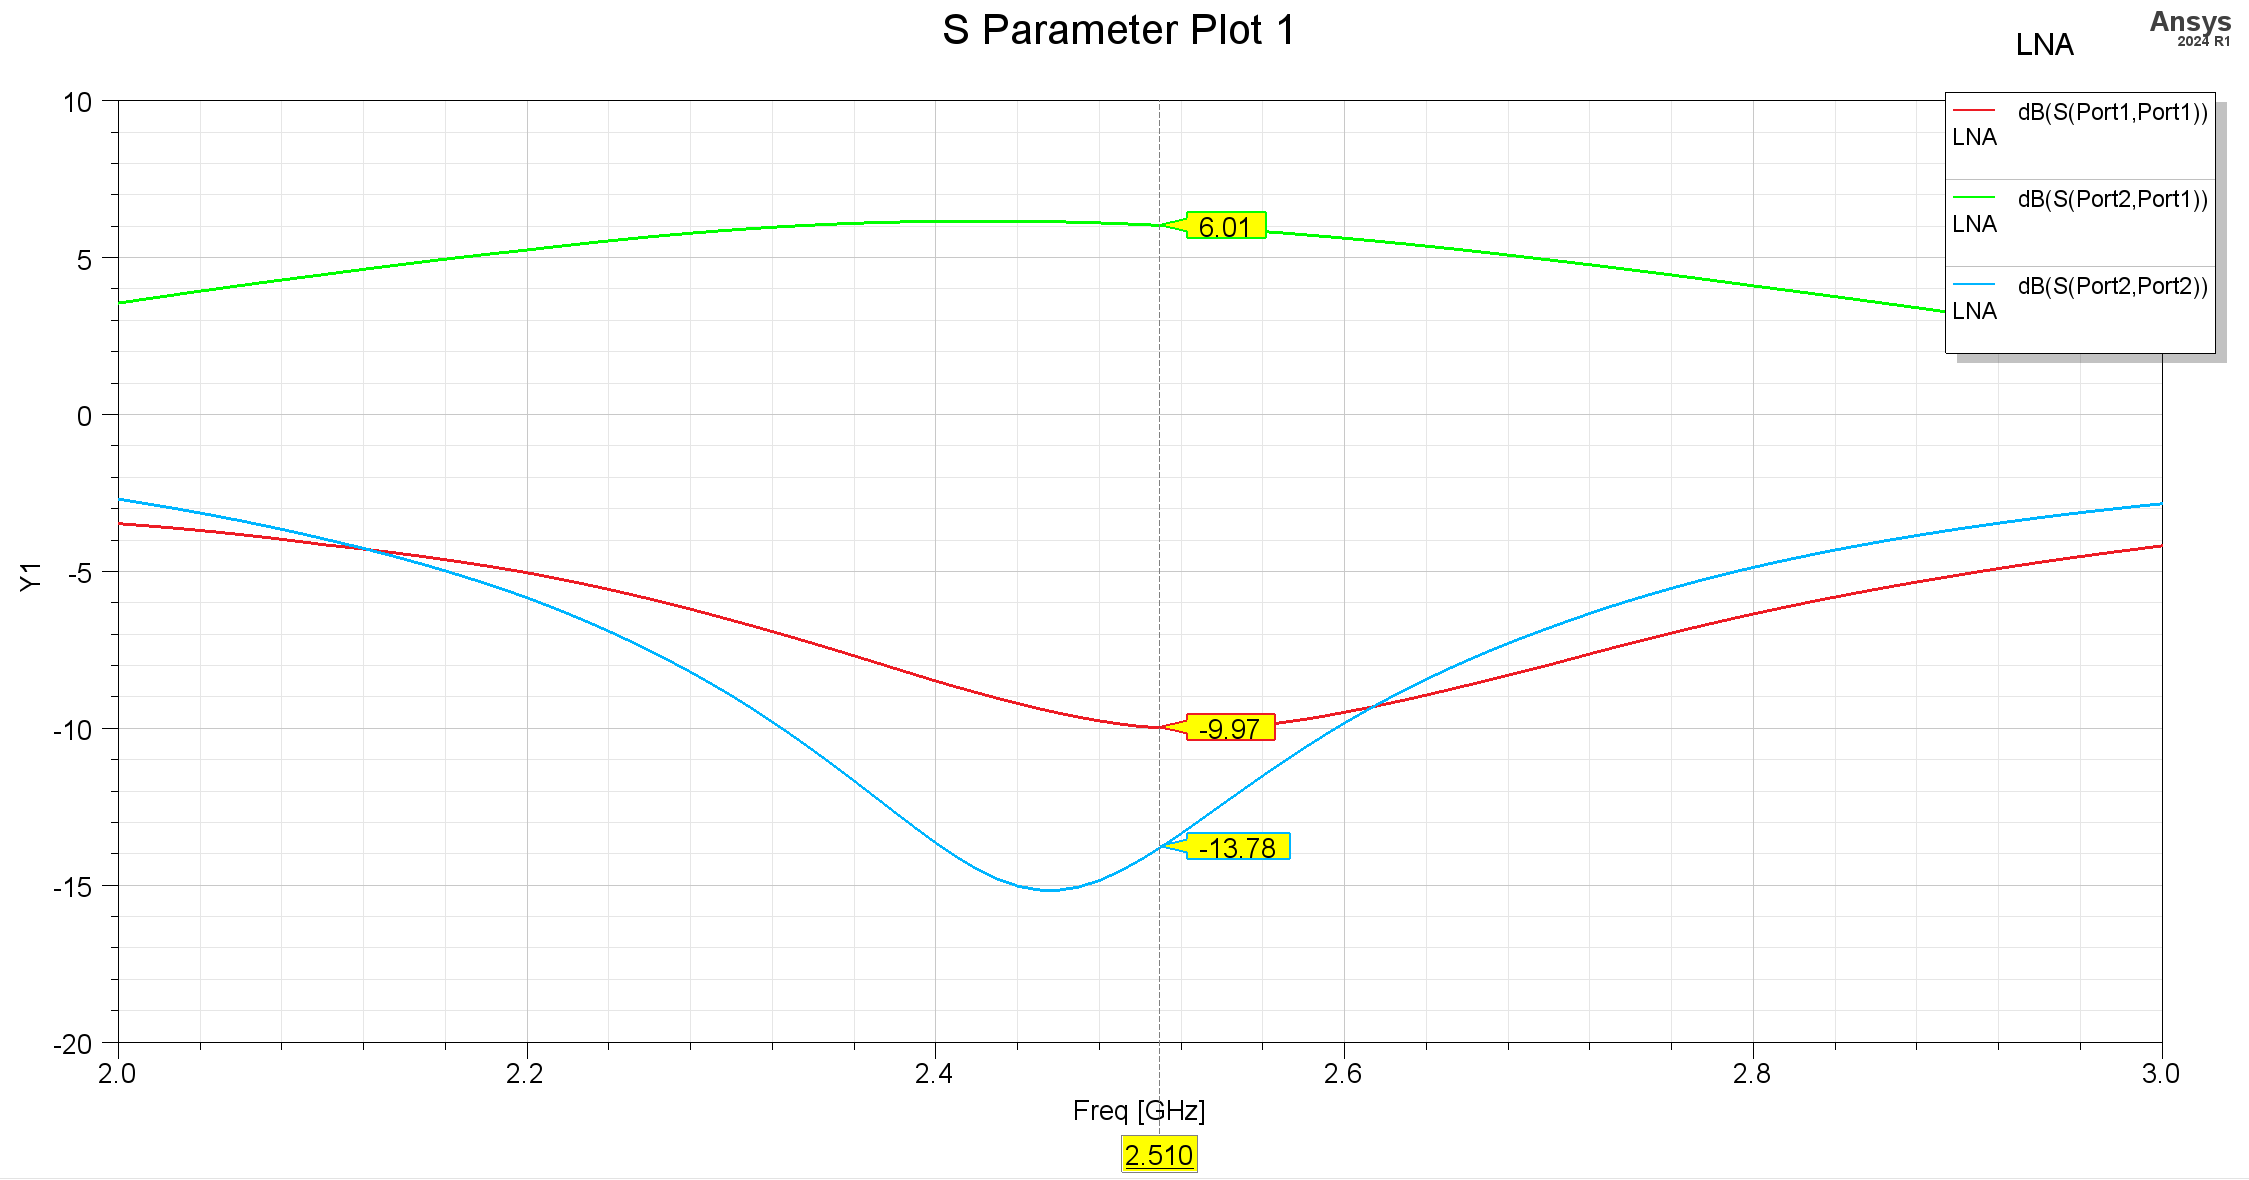
\includegraphics[width=0.8\textwidth]{7.PNG}
	\caption{Частотные характеристики коэффициентов $S_{11}$, $S_{21}$ и $S_{22}$ спроектированного усилителя.}
	\label{fig:results_s_params}
\end{figure}